\chapter{Reti wireless}
Analizzeremo varie tecnologie wireless, quali le LAN wireless, le reti cellulari e le reti d'accesso wireless.
La natura delle LAN wireless è diversa da quella delle LAN cablate, come vedremo in questo capitolo. In Internet sta aumentando l'uso di altre reti wireless come la telefonia cellulare.
Quindi analizzeremo le reti basate su IEEE 802.11, che è lo standard dominante nelle LAN wireless. Poi parleremo delle LAN Bluetooth che vengono usate in molte applicazioni in maniera circoscritta all'utente senza connessione ad Internet.

\section{LAN wireless}
La comunicazione wireless è una tecnologia in forte espansione. La domanda di dispositivi di comunicazione senza l'uso di cavi sta aumentando ovunque. Le reti LAN wireless si possono trovare nei campus universitari, negli uffici e in molte aree pubbliche.

\subsection{Introduzione}
La Figura \ref{fig:componenti-wireless} mostra l’ambiente nel quale considereremo la comunicazione dati wireless e la mobilità. In una rete wireless possiamo identificare i seguenti elementi.

\begin{figure}[ht]
    \centering
    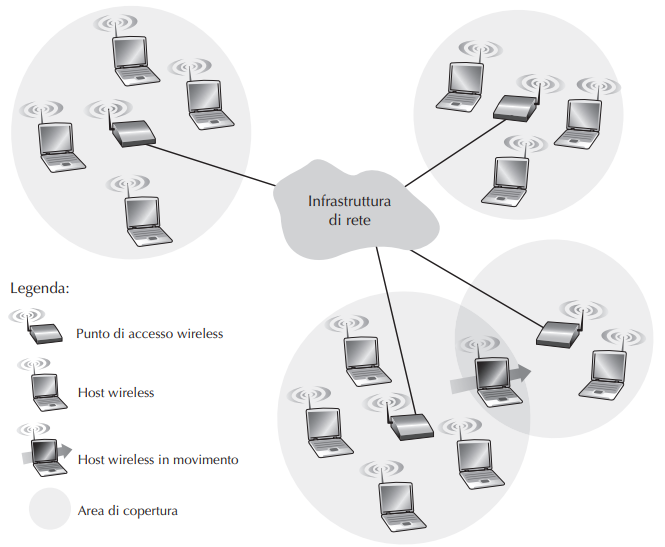
\includegraphics[width=8cm]{images/componenti-wireless.PNG}
    \caption{Componenti di una rete wireless}
    \label{fig:componenti-wireless}
\end{figure}

\begin{itemize}
    \item \textit{Host wireless.} Come nel caso delle reti cablate, gli host sono dispositivi periferici che eseguono applicazioni. L’host wireless può essere un portatile, un tablet, un telefono o un computer desktop. Gli host possono essere mobili o meno.
    \item \textit{Collegamenti wireless.} L’host si connette alla stazione base o a un altro host attraverso un canale di comunicazione wireless. La Figura \ref{fig:caratteristiche-wireless} mostra le due caratteristiche principali (area di copertura e frequenza del collegamento) dei più diffusi standard per collegamenti wireless. 
    
    \begin{figure}[ht]
        \centering
        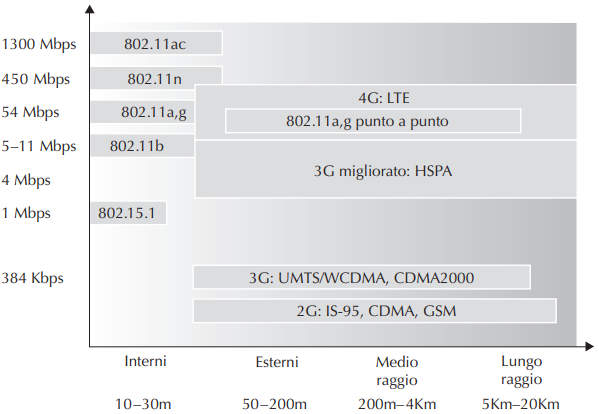
\includegraphics[width=9cm]{images/caratteristiche-wireless.PNG}
        \caption{Caratteristiche dei collegamenti di alcuni standard per reti wireless}
        \label{fig:caratteristiche-wireless}
    \end{figure}
    
    Nella Figura \ref{fig:componenti-wireless} sono illustrati i collegamenti wireless che connettono host collocati alle estremità di una rete. Vedremo che i collegamenti wireless sono utilizzati per connettere router, commutatori e anche altri dispositivi di rete.
    \item \textit{Stazione base (base station).} E' il componente chiave dell’infrastruttura delle reti wireless e, a differenza degli host e dei collegamenti wireless, non ha una controparte corrispondente nelle reti cablate. Una stazione base è responsabile dell’invio e della ricezione dei dati (pacchetti) tra gli host wireless a essa associati. Quando diciamo che un host wireless è “associato” a una stazione base, intendiamo che (1) l’host si trova nell’area di copertura della stazione base e che (2) la utilizza per trasmettere dati verso il resto della rete. Un esempio di queste stazioni base sono i ripetitori di cella (cell tower) nelle reti cellulari e gli access point (punti di accesso) nelle LAN 802.11.

    Nella Figura \ref{fig:componenti-wireless} la stazione base è connessa al resto della rete (per esempio, Internet, rete aziendale, domestica o telefonica) e funziona quindi come ripetitore tra l’host e il resto del mondo con cui comunica. Gli host associati a una stazione base sono considerati come operanti in modalità infrastruttura (infrastructure mode), in quanto tutti i tradizionali servizi di rete (come l’assegnamento degli indirizzi e l’instradamento) sono forniti dalla rete attraverso la stazione base. 
    \item \textit{Infrastruttura di rete.} E' la rete più ampia alla quale l’host wireless potrebbe volersi connettere.
\end{itemize}

\subsubsection{Confronto architetturale}
Per prima cosa confrontiamo l'architettura delle LAN cablate e di quelle wireless per dare un'idea di quali fattori è necessario considerare quando studiamo le LAN wireless.

\begin{itemize}
    \item \textit{Mezzo trasmissivo.} La prima differenza che possiamo osservare tra una LAN cablata e una wireless è il mezzo trasmissivo. Nelle reti cablate usiamo dei cavi per connettere gli host. In una LAN wireless, il mezzo trasmissivo è l'aria e il segnale normalmente è broadcast. Quando gli host in una LAN wireless comunicano l'uno con l'altro, essi condividono lo stesso mezzo (ad accesso multiplo). In una situazione molto rara possiamo creare una comunicazione punto-punto tra due host wireless usando un'ampiezza di banda molto limitata e delle antenne bidirezionali.
    \item \textit{Host wireless.} In una LAN cablata un host è sempre connesso alla sua rete in un punto con un indirizzo MAC fisso che si riferisce alla sua scheda di rete (Network Interface Card, NIC). Naturalmente un host in Internet può spostarsi da un punto all'altro. In questo caso il suo indirizzo MAC rimane lo stesso, ma l'indirizzo IP cambia. Tuttavia, prima che l'host possa usare i servizi di Internet, deve essere fisicamente connesso alla rete. In una LAN wireless, un host non è fisicamente connesso alla rete, ma può muoversi liberamente e usare i servizi da essa forniti.
    \item \textit{LAN isolate.} Anche il concetto di LAN cablata isolata è diverso da quello di LAN wireless isolata. Una LAN cablata isolata è un insieme di host connessi tramite uno switch di collegamento (nella generazione recente dell'Ethernet). Una LAN wireless isolata, chiamata rete ad hoc nella terminologia LAN wireless, è un insieme di host che comunicano liberamente tra loro. Il concetto di switch di collegamento non esiste in questo tipo di rete.

    \begin{figure}[ht]
        \centering
        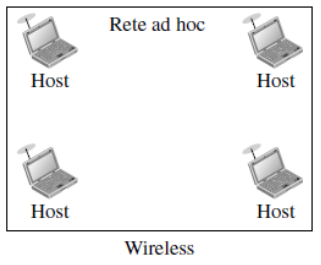
\includegraphics[width=5cm]{images/reti-ad-hoc.PNG}
        \caption{Reti ad hoc}
        \label{fig:reti-ad-hoc}
    \end{figure}
    
    \item \textit{Connessione ad altre reti.} Una LAN cablata si può connettere a un'altra rete o a Internet tramite un router. Una LAN wireless si può connettere a una rete con infrastruttura cablata, a una rete con infrastruttura wireless o a un'altra LAN wireless mediante una base station (stazione base), che nel caso delle reti LAN wireless 802.11 prende il nome di Access Point (AP) o punto di accesso.

    \begin{figure}[ht]
        \centering
        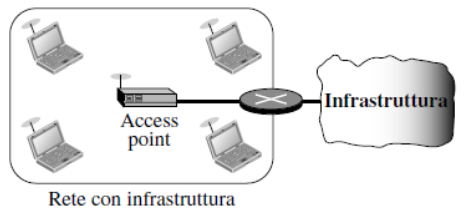
\includegraphics[width=7cm]{images/connessione-wireless.PNG}
        \caption{Connessione di una LAN wireless ad altre reti}
        \label{fig:connessione-wireless}
    \end{figure}

    In questo caso la LAN wireless viene definita rete con infrastruttura (o infrastrutturata) e la connessione all'infrastruttura cablata, come Internet, avviene tramite l'access point, il cui ruolo è completamente diverso da quello di uno switch di collegamento nell'ambiente cablato.
    \item \textit{Migrazione dall'ambiente cablato a quello wireless.} Il funzionamento di una LAN cablata o una wireless dipende dai due livelli inferiori dello stack protocollare TCP/IP. Ciò significa che se abbiamo una LAN cablata in un edificio collegato a Internet tramite un router o un modem, per migrare dall'ambiente cablato a quello wireless è sufficiente cambiare le schede di rete progettate per ambienti cablati con quelle studiate per ambienti wireless e sostituire lo switch di collegamento con un AP. In questo cambiamento anche gli indirizzi MAC si modificheranno (a causa delle NIC diverse), mentre gli indirizzi IP resteranno gli stessi, ci stiamo spostando dai collegamenti cablati a quelli wireless.
\end{itemize}

\subsubsection{Caratteristiche di rete}
Le principali caratteristiche del link wireless sono:
\begin{itemize}
    \item \textit{Attenuazione del segnale.} Le radiazioni elettromagnetiche si attenuano quando attraversano determinati ostacoli (come le pareti delle case). Anche nello spazio libero l’intensità del segnale si attenua al crescere della distanza percorsa (path loss).
    \item \textit{Interferenze da parte di altre sorgenti.} Sorgenti radio che trasmettono nella stessa banda di frequenza interferiscono tra loro. Per esempio, i telefoni a 2,4 GHz e le LAN 802.11b trasmettono nella stessa banda di frequenze. Quindi, gli utenti della LAN 802.11b che parlano con un telefono wireless a 2,4 GHz non devono sorprendersi se rete e telefono presentano malfunzionamenti. Inoltre il rumore elettromagnetico ambientale (per esempio, di un motore o di un forno a microonde) può generare interferenze.
    \item \textit{Propagazione su più cammini (multipath propagation).} La propagazione su più cammini si verifica quando una parte delle onde elettromagnetiche si riflette su oggetti e sul terreno, percorrendo cammini di diversa distanza tra il trasmittente e il ricevente. Questo fenomeno disturba il segnale che giunge al destinatario. Oggetti in movimento tra il trasmittente e il ricevente possono causare il fenomeno di propagazione multipla, che varia in ogni momento.
\end{itemize}

Quanto osservato fin qui suggerisce che gli errori nei bit siano più frequenti nei collegamenti wireless che nelle reti cablate. Per questo motivo non dobbiamo sorprenderci se i protocolli di collegamento wireless utilizzano non solo potenti codici CRC di rilevazione degli errori, ma anche un protocollo di trasferimento affidabile a livello di
collegamento, che ritrasmette i pacchetti danneggiati.

Dopo aver considerato i deterioramenti che possono avvenire in un canale wireless, rivolgiamo la nostra attenzione agli host che ricevono il segnale. Questi host ricevono un segnale elettromagnetico che è la combinazione di una forma degradata del segnale originale trasmesso dal mittente (degradato, per esempio, a causa degli effetti dell’attenuazione e della propagazione su cammini multipli) e un rumore di fondo dell’ambiente. Il rapporto segnale rumore (SNR, signal-to-noise ratio) è una misura relativa dell’intensità del segnale ricevuto, cioè dell’informazione che è stata trasmessa, e del rumore. Per i nostri scopi, ci basti sapere che un SNR più grande facilita il ricevente nel distinguere il segnale trasmesso dal rumore di fondo.

\subsubsection{Controllo dell'accesso al mezzo}
Forse il problema più importante di cui dobbiamo parlare in una LAN wireless è il controllo d'accesso, ovvero come un host wireless può avere accesso al mezzo di trasmissione condiviso (aria). Abbiamo detto che l'Ethernet Standard usava l'algoritmo CSMA/CD. Secondo tale metodo ogni host compete per accedere al mezzo e trasmette il suo frame se il mezzo è inattivo. Se avviene una collisione, essa viene rilevata e il frame inviato nuovamente. Il rilevamento delle collisioni nel CSMA/CD ha due scopi. Il fatto che venga rilevata una collisione significa che il frame non è stato ricevuto e deve essere inviato nuovamente. Se invece non viene rilevata alcuna collisione, allora vuol dire che il frame è stato ricevuto correttamente. L'algoritmo CSMA/CD non funziona nelle LAN wireless per tre ragioni.
\begin{enumerate}
    \item Per rilevare una collisione un host deve poter inviare (il proprio frame) e ricevere (ascoltare il canale per capire se qualcun altro sta trasmettendo) contemporaneamente, il che significa che l'host deve operare in modalită duplex. Poiché la potenza del segnale ricevuto è molto inferiore a quella del segnale trasmesso, sarebbe troppo costoso impiegare un adattatore di rete in grado di rilevare collisioni (i dispositivi wireless hanno un'energia limitata, fornita dalla batteria, che non gli consente di utilizzare un tale dispositivo). Pertanto i dispositivi wireless non possono rilevare le collisioni (Collision Detection) come avviene per Ethernet.
    \item A causa del problema del terminale nascosto (hidden terminal problem) secondo cui un host, nel seguito chiamato anche terminale o stazione, potrebbe non sapere che un altro host sta trasmettendo a causa di ostacoli o questioni dovute al raggio di trasmissione - una collisione potrebbe avvenire senza essere rilevata. 

    \begin{Example}{Problema del terminale nascosto}{}
        \textit{La figura mostra un esempio del problema del terminale nascosto.}

        \begin{minipage}{\textwidth}
            \centering
            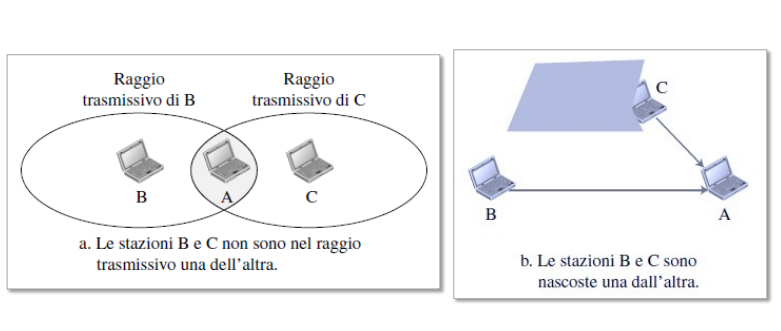
\includegraphics[width=0.8\textwidth]{images/problema-terminale-nascosto.PNG}
            %\captionof{figure}{Esempio}
        \end{minipage}
        
        Il raggio di trasmissione dell'host B è mostrato dall'ovale sinistro (sfera nello spazio); ogni host all'interno di tale raggio può sentire i segnali trasmessi da B. Analogamente, il raggio di trasmissione della stazione C è indicato con l'ovale destro (sfera nello spazio); ogni host situato entro tale raggio riceve i segnali trasmessi da C. L'host C è all'esterno del raggio di trasmissione di B; allo stesso modo B è all'esterno del raggio di C. L'host A, tuttavia, si trova nell'area coperta sia da B che da C quindi può sentire qualsiasi segnale trasmesso da B o da C. La figura mostra inoltre che il problema del terminale nascosto può presentarsi anche a causa di un ostacolo.

        Supponiamo che B stia inviando dei dati ad A. Nel bel mezzo della trasmissione, anche C ha dei dati da inviare ad A. Tuttavia, C è fuori dal raggio di B e le trasmissioni di B non possono raggiungere C. Quindi C crede che il mezzo sia libero, e invia i suoi dati ad A, il che risulta in una collisione su A in quanto tale host si trova a ricevere dei dati sia da B che da C. In questo caso possiamo dire che i terminali B e C sono nascosti tra loro rispetto ad A. I terminali nascosti possono ridurre la capacità della rete a causa della possibilità di collisioni.
    \end{Example}
    
    \item La distanza tra gli host può essere grande. L'attenuazione del segnale può impedire a un host di sentire una collisione che avviene ad un'altra estremità.
\end{enumerate}

\subsection{IEEE 802.11}
L'IEEE ha definito le specifiche per le LAN wireless, chiamate IEEE 802.11, che copre i livelli fisico e di collegamento. In alcune nazioni, compresi gli Stati Uniti, si usa il termine Wi-Fi (abbreviazione di wireless fidelity) come sinonimo di LAN wireless. Wi-Fi è una LAN wireless certificata dalla Wi-Fi Alliance, un'associazione industriale globale no-profit, di cui fanno parte oltre 300 aziende, che si occupa di promuovere la crescita delle LAN wireless.

\subsubsection{Architettura}
Lo standard IEEE 802.11 definisce due tipi di architetture: il basic service set (BSS) e l'extended service set (ESS). L'architettura basic service set (BSS) è costituita da una o più stazioni wireless (dette anche host, dispositivi, nodi) e da un access point facoltativo. La Figura \ref{fig:bss} mostra due BSS di questo standard.

\begin{figure}[ht]
    \centering
    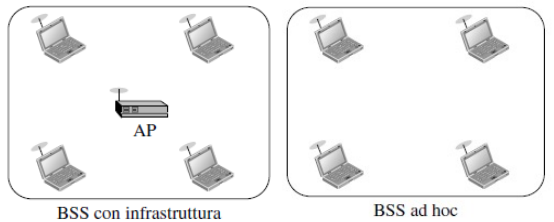
\includegraphics[width=7cm]{images/bss.PNG}
    \caption{Basic service set (BSS)}
    \label{fig:bss}
\end{figure}

Il secondo tipo di architettura, l'extended service set (ESS), è costituito da due o più BSS con infrastruttura. In questo caso i BSS sono collegati tramite un sistema di distribuzione, che è una rete cablata o wireless. Il sistema di distribuzione collega gli AP nei BSS. L'IEEE 802.11 non limita il sistema di distribuzione, può essere una LAN IEEE come ad esempio una Ethernet. La Figura \ref{fig:ess} illustra un ESS.

\begin{figure}[ht]
    \centering
    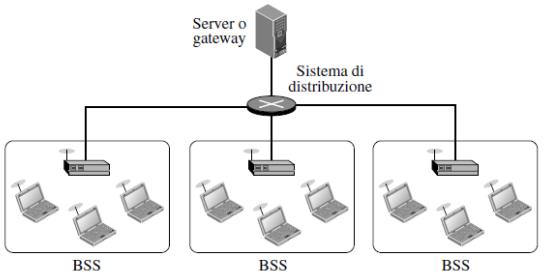
\includegraphics[width=9cm]{images/ess.PNG}
    \caption{Extended service set (ESS)}
    \label{fig:ess}
\end{figure}

Quando i BSS sono collegati, le stazioni che si possono raggiungere a vicenda (in visibilità) comunicano senza l'uso di un AP. Tuttavia, la comunicazione tra una stazione in un BSS e una al suo esterno avviene tramite l'AP. 

Prima di inviare o ricevere pacchetti dati 802.11 le stazioni devono associarsi a un AP. Quando un amministratore di rete installa un AP, gli assegna uno o due identificativi, detti SSID (service set identifier). L’amministratore deve anche assegnare all’AP un numero di canale. Per comprendere questo concetto ricordiamo che 802.11 opera nella banda di frequenza da 2,4 GHz a 2,4835 GHz. In questi 85 MHz di banda, 802.11 definisce 11 canali parzialmente sovrapposti. Due canali non si sovrappongono solo se sono separati da quattro o più canali. In particolare, i canali 1, 6 e 11 costituiscono l’unica terna priva di sovrapposizione. Questo significa che un amministratore potrebbe creare una LAN wireless con una capacità trasmissiva globale di 33 Mbps, installando tre AP 802.11b nello stesso luogo, assegnando i canali 1, 6 e 11 agli AP e connettendoli con uno switch.

L'architettura IEEE 802.11 prevede che una stazione wireless si associ a un AP per accedere a Internet. Sorge dunque il problema di conoscere quali AP sono disponibili in un BSS e come avviene l'associazione. Lo standard 802.11 prevede che un AP invii dei segnali periodici, detti beacon, che includono l'identificatore dell'AP (Service Set Identifier - SSID) e il suo indirizzo MAC. La stazione wireless che vuole entrare in un BSS, scandisce gli 11 canali trasmissivi alla ricerca di frame beacon (passive scanning). Alla fine della scansione la stazione sceglie l'AP da cui ha ricevuto il beacon con la maggiore potenza di segnale e gli invia un frame con la richiesta di associazione. L'AP accetta l'associazione rispondendo con un frame di risposta di associazione, che permetterà all'host entrante di inviare una richiesta DHCP per ottenere un indirizzo IP nella rete.

La richiesta di associazione verso un particolare AP può avvenire mediante una fase di autenticazione: l'AP può richiedere alla stazione di autenticarsi mediante un nome utente e una password. Oppure l'autenticazione può avvenire in base all'indirizzo MAC della stazione. Una volta eseguita l'associazione, la stazione wireless può comunicare con l'AP per inviare e ricevere traffico anche verso/da Internet. Tuttavia, più stazioni possono voler trasmettere frame nello stesso momento, per cui è necessario regolare l'accesso al canale con un protocollo MAC che coordini le trasmissioni.

\subsubsection{Protocollo MAC 802.11}
L'IEEE 802.11 definisce due tecniche di accesso al mezzo: una distribuita (distributed coor dination function - DCF) in cui i nodi si contendoro l'accesso al canale, e un'altra centralizzata (point coordination function - PCF), in cui non c'è contesa e l'AP coordina l'accesso dei nodi al canale. In questo testo ci concentriamo sulla prima tecnica.

La tecnica Distributed Coordination Function (DCF) usa il protocollo CSMA/CA come metodo d'accesso. Poiché nelle reti wireless la rilevazione delle collisioni (collision detection) non può essere eseguita durante la trasmissione, è stato definito il protocollo di Carrier Sense Multiple Access with Collision Avoidance (CSMA/CA) che ha lo scopo di evitare che si verifichino collisioni.

Al contrario del protocollo Ethernet 802.3, il protocollo MAC 802.11 non implementa la rilevazione delle collisioni. Esistono due fondamentali ragioni per questa scelta.
\begin{itemize}
    \item La possibilità di rilevare collisioni richiede la capacità di inviare (il segnale proprio della stazione) e ricevere (per determinare se un’altra stazione sta anch’essa trasmettendo) contemporaneamente. Essendo in genere la potenza del segnale ricevuto nettamente inferiore alla potenza del segnale trasmesso dall’adattatore 802.11, risulta molto costoso costruire hardware che possa rilevare una collisione.
    \item Estremamente più significativo è il fatto che l’adattatore, anche se fosse in grado di trasmettere e ricevere allo stesso istante (presumibilmente interrompendo la trasmissione quando trova il canale occupato), non potrebbe rilevare tutte le collisioni a causa del problema del terminale nascosto e dell’attenuazione del segnale.
\end{itemize}

Ricordiamo che un frame inviato da una stazione in una rete wireless potrebbe non raggiungere la stazione di destinazione per numerosi motivi. Per contrastare queste non trascurabili possibilità di fallimento, MAC 802.11 utilizza la conferma di avvenuta ricezione a livello di collegamento. Come mostrato nella Figura \ref{fig:ack-802.11}, quando la stazione di destinazione riceve un frame che passa il controllo CRC, attende per un breve periodo di tempo, noto come SIFS (short inter-frame space, spazio breve inter-frame), dopo il quale invia al mittente un frame di conferma di avvenuta ricezione. Se la stazione trasmittente non riceverà questo riscontro entro un arco di tempo stabilito, presupporrà un errore e ritrasmetterà il frame, utilizzando ancora il protocollo CSMA/CA per accedere al canale. Se il frame di conferma non sarà ricevuto dopo un numero prefissato di ritrasmissioni, la stazione trasmittente passerà oltre e scarterà il frame.

\begin{figure}[ht]
    \centering
    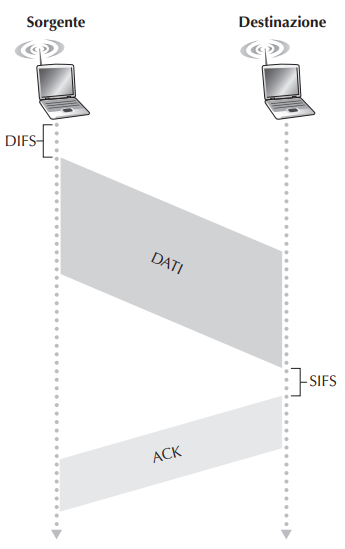
\includegraphics[width=6cm]{images/ack-802.11.PNG}
    \caption{IEEE 802.11 usa acknowledgment a livello di collegamento}
    \label{fig:ack-802.11}
\end{figure}

Prima di tutto vengono evitate le collisioni rimandando la trasmissione anche se il canale viene trovato libero: rilevata la portante, se il canale risulta libero, la stazione non trasmette immediatamente, ma attende un lasso di tempo chiamato interframe space o IFS. La motivazione di questa scelta sta nel fatto che il canale può apparire inattivo quando viene rilevato, ma una stazione distante può avere già iniziato a trasmettere. Il segnale della stazione distante non ha ancora raggiunto la stazione in oggetto. Il tempo IFS consente alla prima parte del segnale trasmesso dalla stazione distante di raggiungere la stazione che vuole trasmettere. Dopo aver atteso per un tempo IFS, se il canale è ancora inattivo, la stazione prima di trasmettere deve attendere un tempo di back-off, equivalente al tempo di contesa.

\begin{enumerate}
    \item Se inizialmente la stazione percepisce il canale come inattivo, allora trasmette il suo frame dopo un breve periodo di tempo conosciuto come DIFS (distributed inter-frame space, spazio distribuito inter-frame).
    \item Altrimenti, la stazione sceglie un valore casuale di ritardo usando una attesa binaria esponenziale e decrementa questo valore dopo DIFS solo quando il canale viene percepito come inattivo. Se il canale è percepito come occupato, il contatore rimane fermo.
    \item Quando il contatore arriva a zero (notiamo che questo può verificarsi soltanto quando il canale è percepito come inattivo), la stazione trasmette l’intero frame e aspetta il frame di conferma.
    \item Se riceve la conferma, la stazione sa che il frame è stato ricevuto correttamente e, qualora avesse un altro frame da inviare, riattiva il protocollo CSMA/CA dal passo 2. Se il frame di conferma non viene ricevuto, la stazione trasmittente ritorna al passo 2, ma con un valore di ritardo maggiore.
\end{enumerate}

La finestra di contesa consiste di un lasso di tempo diviso in slot, detto back-off time. Una stazione che vuole trasmettere sceglie come tempo di attesa una quantità casuale di slot (back-off timer). Il numero di slot nella finestra cambia ad ogni trasmissione di un nuovo frame in base alla strategia di back-off binario esponenziale. Ciò significa che la prima volta il back-off viene impostato a uno slot e poi raddoppia ogni volta che la stazione non riesce a ottenere accesso al canale o a trasmettere con successo il frame. Un aspetto interessante della finestra di contesa è che la stazione deve ascoltare il canale dopo ogni slot di tempo: se trova il canale occupato, interrompe il timer e lo riavvia quando il canale viene rilevato libero.

\begin{figure}[ht]
    \centering
    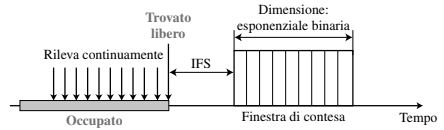
\includegraphics[width=9cm]{images/finestra-contesa.PNG}
    \caption{Finestra contesa}
    \label{fig:finestra-contesa}
\end{figure}

Poiché questi meccanismi non garantiscono che non avvenga una collisione, è necessario utilizzare riscontri positivi e timer per capire se la trasmissione del frame è andata a buon fine.

\begin{Example}{Modello temporale dello scambio di frame}{}
    \textit{La figura illustra lo scambio dei frame di controllo e di dati nel tempo.}

    \begin{minipage}{\textwidth}
        \centering
        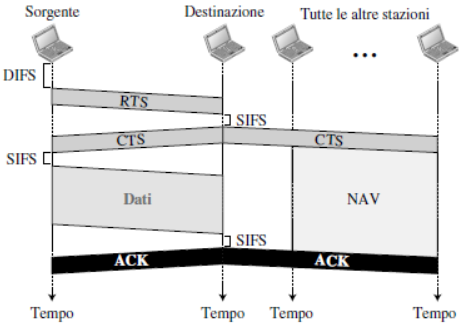
\includegraphics[width=0.6\textwidth]{images/csma-nav.PNG}
        %\captionof{figure}{Esempio}
    \end{minipage}

    \begin{enumerate}
    \item Prima di inviare un frame la stazione sorgente ascolta il canale controllando il livello d'energia sulla frequenza portante. La stazione usa una strategia di persistenza con back-off finché il canale non è libero. Dopo che il canale viene rilevato inattivo, la stazione attende per un lasso di tempo chiamato DCF interframe space (DIFS), quindi invia un frame di controllo chiamato request to send (RTS), che indica la volontà di spedire un frame.
    \item Dopo aver ricevuto l'RTS e aver atteso per un lasso di tempo chiamato short interframe space (SIFS), la stazione di destinazione invia un frame di controllo, chiamato clear to send (CTS) alla stazione sorgente, che indica che la stazione di destinazione è pronta a ricevere i dati.
    \item La stazione sorgente attende un lasso di tempo pari al SIFS, dopodiché invia i dati.
    \item La stazione di destinazione, dopo aver atteso un lasso di tempo pari al SIFS, invia un riscontro (ack) per mostrare che il frame è stato ricevuto. Il riscontro è necessario in tale protocollo in quanto la stazione sorgente non ha alcun mezzo per verificare l'effettivo arrivo dei suoi dati a destinazione.
    \end{enumerate}
\end{Example}

Se una stazione acquisisce l'accesso, come fanno le altre a posticipare l'invio dei loro dati? In altre parole, come si evita la collisione in questo protocollo? La chiave è una caratteristica chiamata NAV.

Quando una stazione invia un frame RTS include la durata di tempo in cui occuperà il canale per trasmettere il frame e ricevere l'ack. Le stazioni che sono influenzate da tale trasmissione avviano un timer chiamato network allocation vector (NAV) che indica quanto tempo deve passare prima che possano verificare l'inattività del canale. Ogni volta che una stazione accede al sistema ed invia un frame RTS le altre stazioni avviano i loro NAV. In altre parole ogni stazione, prima di ascoltare il canale per vedere se è inattivo, verifica che il suo NAV sia scaduto.

Che cosa accade se avviene una collisione durante il tempo in cui i frame di controllo RTS o CTS sono in transizione, spesso definito periodo di handshaking? Due o più stazioni possono cercare di inviare dei frame RTS contemporaneamente. Questi frame di controllo possono collidere. Tuttavia, siccome non c'è meccanismo per rilevare la collisione, il mittente suppone che ci sia stata una collisione se non ha ricevuto un frame CTS dal destinatario. Viene quindi applicata la strategia del back-off e il mittente prova di nuovo.

La soluzione al problema del terminale nascosto è l'uso dei frame RTS e CTS. 

\begin{Example}{Problema del terminale nascosto}{}
    \textit{La figura mostra anche che il messaggio RTS da B raggiunge A, ma non C.}

    \begin{minipage}{\textwidth}
        \centering
        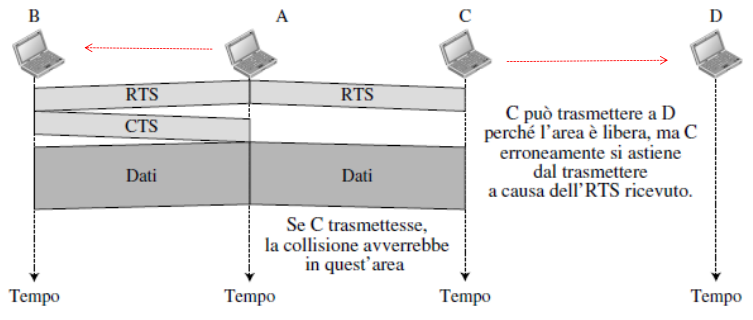
\includegraphics[width=0.6\textwidth]{images/prob-terminale-nascosto.PNG}
        %\captionof{figure}{Esempio}
    \end{minipage}
    
    Tuttavia, siccome sia B che C si trovano entro il raggio di A, il messaggio CTS, che contiene la durata della trasmissione dei dati da B ad A, raggiunge C. La stazione C capisce quindi che c'è una trasmissione che interessa uno dei suoi vicini e si astiene dall'invio sino alla fine della trasmissione.    
\end{Example}

Il frame di livello MAC è costituito da nove campi, come mostrato nella Figura \ref{fig:formato-frame}.

\begin{figure}[ht]
    \centering
    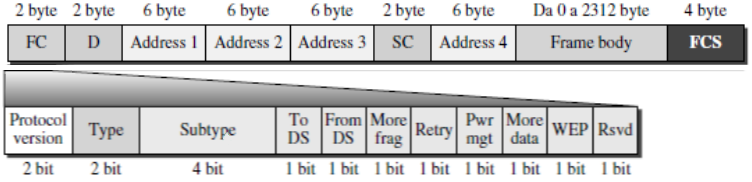
\includegraphics[width=11cm]{images/formato-frame.PNG}
    \caption{Formato del frame}
    \label{fig:formato-frame}
\end{figure}

\begin{itemize}
    \item \textit{Frame Control (FC).} Il campo FC è lungo 2 byte e definisce il tipo di frame e alcune informazioni di controllo.
    \item \textit{D.} Questo campo definisce la durata della trasmissione che viene usata per impostare il valore del NAV. In un frame di controllo esso definisce l'ID del frame.
    \item \textit{Indirizzi.} Ci sono quattro campi indirizzo, ognuno lungo 6 byte. Il significato di ogni campo dipende dal valore dei sottocampi To DS e From DS che verranno analizzati in seguito.
    \item \textit{SC (controllo sequenza).} Questo campo definisce un valore da 16 bit. I primi quattro bit indicano il numero del frammento e gli ultimi 12 quello della sequenza, che è la stessa in tutti i frammenti.
    \item \textit{Frame body (corpo del frame).} Questo campo, che può essere da 0 a 2312 byte, contiene le informazioni sulla base del tipo e del sotto-tipo definito nel capo FC.
    \item \textit{FCS.} Il campo FCS è lungo 4 byte e contiene una sequenza CRC-32 di rilevamento errori.
\end{itemize}

Una LAN wireless definita dall'IEEE 802.11 ha tre categorie di frame: gestione, controllo e dati.
\begin{itemize}
    \item \textit{Frame di gestione.} Vengono usati per la comunicazione iniziale tra stazioni e punti d'accesso. Per i frame di gestione il valore del campo tipo è 00.
    \item \textit{Frame di controllo.} Si usano per accedere al canale e dare riscontro ai frame. Per i frame di controllo il valore del campo tipo è 01; i valori dei campi sotto-tipo per i frame di cui abbiamo parlato sono 1011:RTS, 1100:CTS, 1101:ACK.
    \item \textit{Frame di dati.} Vengono usati per trasportare i dati e le informazioni di controllo.
\end{itemize}

\begin{figure}[ht]
    \centering
    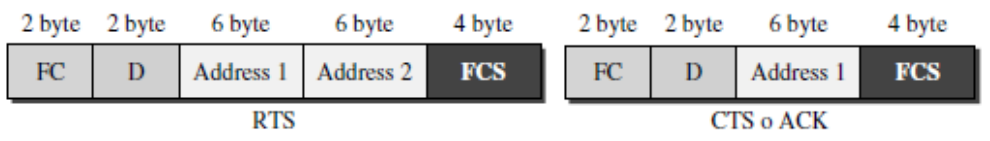
\includegraphics[width=11cm]{images/frame-di-controllo.PNG}
    \caption{Frame di controllo}
    \label{fig:frame-di-contrllo}
\end{figure}

\subsubsection{Indirizzamento}
Il meccanismo d'indirizzamento dell'IEEE 802.11 specifica quattro casi, definiti dal valore dei due flag nel campo FC, To DS e From DS. Ogni flag può essere 0 o 1, di conseguenza possiamo avere quattro situazioni diverse. L'interpretazione dei quattro indirizzi (da 1 a 4) nel frame MAC dipende dal valore di tali flag.

\begin{table}[ht]
    \centering
    \begin{tabular}{|c|c|c|c|c|c|}
         \hline
         \textit{To DS} & \textit{From DS} & \textit{Address 1} & \textit{Address 2} & \textit{Address 3} & \textit{Address 4}\\\hline
         0&0 & Destinazione & Sorgente & DSS ID & N/A\\\hline
         0&1 & Destinazione & AP mittente & Sorgente & N/A\\\hline
         1&0 & AP ricevente & Sorgente & Destinazione & N/A\\\hline
         1&1 & AP ricevente & AP mittente & Destinazione & Sorgente\\\hline
    \end{tabular}
    \caption{Indirizzi}
    \label{tab:indirizzi}
\end{table}

Da notare che l'indirizzo 1 è sempre quello del dispositivo successivo che verrà visitato dal frame. L'indirizzo 2 è sempre quello del dispositivo precedente che il frame ha lasciato. L'indirizzo 3 è quello della stazione di destinazione finale se non viene definito dall'indirizzo 1 o quello della stazione sorgente originale se non è definito dall'indirizzo 2. L'indirizzo 4 è la sorgente originale quando anche il sistema di distribuzione è wireless.
\begin{itemize}
    \item \textit{Caso 00.} In questo caso \textit{To DS = 0} e \textit{From DS = 0}. Ciò significa che il frame non sta andando verso un sistema di distribuzione (\textit{To DS = 0}) e non sta arrivando da uno di essi (\textit{From DS = 0}). Esso sta andando da una stazione in un BSS verso un'altra senza passare dal sistema di distribuzione.
    \item \textit{Caso 01.} In questo caso \textit{To DS = 0} e \textit{From DS = 1}. Ciò significa che il frame arriva da un sistema di distribuzione (\textit{From DS = 1}). Esso giunge da un AP e si dirige verso una stazione. Da notare che l'indirizzo 3 contiene il mittente originale del frame (in un altro BSS).
    \item \textit{Caso 10.} In questo caso \textit{To DS = 1} e \textit{From DS = 0}. Ciò significa che il frame sta andando verso un sistema di distribuzione (\textit{To DS = 1}). Esso va da una stazione a un AP. L'ACK viene inviato alla stazione originale. Da notare che l'indirizzo 3 contiene la destinazione finale del frame nel sistema di distribuzione.
    \item \textit{Caso 11.} In questo caso \textit{To DS = 1} e \textit{From DS=1}. Questo è il caso in cui anche il sistema di distribuzione è wireless. Il frame sta andando da un AP a un altro AP in un sistema di distribuzione wireless. Qui servono quattro indirizzi per definire il mittente originale, la destinazione finale e due AP intermedi.
\end{itemize}

\begin{figure}[ht]
    \centering
    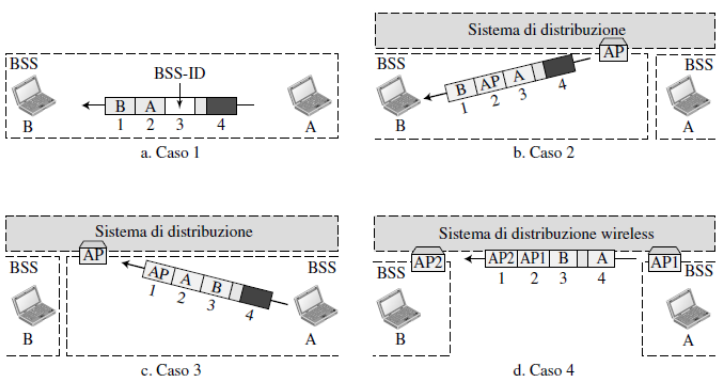
\includegraphics[width=11cm]{images/meccanismo-indirizzamento.PNG}
    \caption{Meccanismo d'indirizzamento}
    \label{fig:meccanismo-indirizzamento}
\end{figure}

\subsubsection{Mobilità all’interno di una sottorete IP}
Per aumentare la copertura di una LAN wireless, aziende e università dispongono spesso vari BSS all’interno di una stessa sottorete IP. Questo naturalmente fa nascere il problema della mobilità all’interno dei BSS: come può una stazione wireless muoversi da un BSS a un altro durante la stessa sessione TCP? Come vedremo ora, la mobilità può essere trattata in modo semplice quando i BSS fanno parte di una stessa sottorete.

\begin{Example}{Mobilità all'interno della stessa sottorete}{}
    \textit{La figura mostra due BSS interconnessi con l’host H1, che si sposta da BSS1 a BSS2.}

    \begin{minipage}{\textwidth}
        \centering
        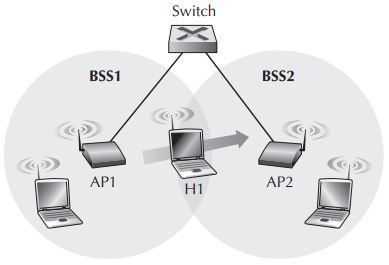
\includegraphics[width=0.5\textwidth]{images/mobilità-sottorete.PNG}
        %\captionof{figure}{Esempio}
    \end{minipage}
    
    Dato che in questo esempio il dispositivo che connette i due BSS non è un router, tutte le stazioni all’interno di queste, inclusi gli AP, apparterranno alla stessa sottorete IP. Quindi, quando H1 si sposta da BSS1 a BSS2, può mantenere il suo indirizzo IP e tutte le sue connessioni TCP aperte. Se il dispositivo d’interconnessione fosse stato un router, allora H1 avrebbe dovuto cambiare l’indirizzo IP e chiudere tutte le connessioni TCP, oppure usare un protocollo di mobilità a livello di rete come, per esempio, IP mobile.

    Ma, in dettaglio, che cosa accade quando H1 si sposta da BSS1 a BSS2? Man mano che H1 si allontana da AP1, ne riceve sempre più debolmente il segnale e inizia a ricercarne uno più intenso di un altro access point. H1 riceve i frame beacon da AP2 che, come spesso avviene, avrà lo stesso SSID di AP1. Quindi H1 si disconnette da AP1 e si associa ad AP2, mentre mantiene il suo indirizzo IP e le sue connessioni TCP aperte.

    Questo risolve il problema dell’handoff dal punto di vista dell’host e dell’AP. Ma come fa uno switch a sapere che l’host si è spostato da un AP a un altro? Come ricorderete, gli switch auto-apprendono, costruendo automaticamente le proprie tabelle d’inoltro. Grazie a questa qualità di auto-apprendimento si riescono ad affrontare positivamente spostamenti occasionali (per esempio, quando un impiegato si sposta da un ufficio a un altro); ma gli switch non sono stati progettati per supportare utenti che si spostano di frequente, pretendendo di mantenere le loro connessioni TCP mentre cambiano BSS. Per valutare questo problema, ricordiamo che prima dello spostamento, lo switch ha una voce nella sua tabella d’inoltro che associa l’indirizzo MAC di H1 alla porta attraverso la quale H1 può essere raggiunto. Se H1 è inizialmente in BSS1, allora il datagramma destinato a H1 gli sarà inoltrato attraverso l’AP1. Una volta che H1 si sarà associato a BSS2, comunque, il suo frame dovrebbe essere diretto ad AP2. Una soluzione (un trucco, in realtà) potrebbe essere che, appena realizzata la nuova associazione, AP2 invii in broadcast allo switch un frame Ethernet, con l’indirizzo sorgente di H1. Ricevuto il frame, lo switch aggiornerà la sua tabella d’inoltro, in modo che H1 sia raggiungibile attraverso AP2.    
\end{Example}

\subsection{Bluetooth}
Il Bluetooth è una tecnologia LAN wireless progettata per connettere dispositivi con diverse funzioni, come telefoni, notebook, computer (desktop e laptop), macchine fotografiche, stampanti e anche macchinette del caffè quando si trovano a una breve distanza l'una dall'altra. Una LAN Bluetooth è una rete ad hoc, il che significa che si forma spontaneamente, senza l'aiuto di alcuna stazione base (access point); i dispositivi si accordano l'un l'altro e creano una rete chiamata piconet, che può essere composta al massimo da 8 dispositivi. Una LAN Bluetooth può essere connessa persino a Internet se uno dei dispositivi ha tale capacità. Essa però, per natura, non può essere grande. Se ci sono molti dispositivi che cercano di connettersi si crea il caos.

Il Bluetooth originariamente è stato avviato come progetto dalla società Ericsson. Il suo nome deriva da Harald Blaatand, re di Danimarca (940-981) che unì Danimarca e Norvegia Blaatand tradotto in inglese significa Bluetooth.

Oggigiorno la tecnologia Bluetooth è l'implementazione di un protocollo definito dallo standard IEEE 802.15. Lo standard definisce una rete wireless di area personale (PAN) funzionante in un'area delle dimensioni di una stanza. I dispositivi Bluetooth sono a bassa potenza, hanno una portata di 10 m, e usano una banda ISM da 2,4 GHz divisa in 79 canali da 1 MHz ciascuno.

\subsubsection{Architettura}
Il Bluetooth delinea due tipi di rete: la piconet e la scatternet.

Una rete Bluetooth viene chiamata piconet, o piccola rete. Essa può avere fino a otto stazioni, una delle quali è detta primaria (master), e le altre sono secondarie (slave). Tutte le stazioni secondarie sincronizzano i loro orologi e le sequenze di hopping con la stazione primaria. Da notare che una piconet può avere una sola stazione primaria. La comunicazione tra la stazione primaria e le secondarie può essere uno-a-uno o uno-a-molti.

\begin{figure}[ht]
    \centering
    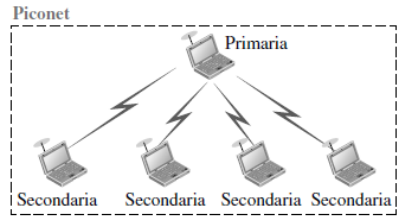
\includegraphics[width=7cm]{images/piconet.PNG}
    \caption{Piconet}
    \label{fig:piconet}
\end{figure}

Anche se una piconet può avere un massimo di sette stazioni secondarie, altre possono essere in stato parked (in sosta). Una stazione secondaria in stato parked è sincronizzata con la primaria, ma non può prendere parte alla comunicazione finché non viene spostata dallo stato parked allo stato attivo. Siccome solo otto stazioni possono essere attive in una piconet, attivare una stazione da uno stato parked significa che una stazione attiva deve andare in tale stato.

Le piconet si possono combinare per formare quella che viene definita una scatternet. Una stazione secondaria in una piconet può essere la primaria in un'altra piconet. Tale stazione può ricevere dei messaggi dalla stazione primaria nella prima piconet (come secondaria) e, agendo da primaria, consegnarli alle stazioni secondarie nella seconda piconet. Una stazione può appartenere a due piconet. 

\begin{figure}[ht]
    \centering
    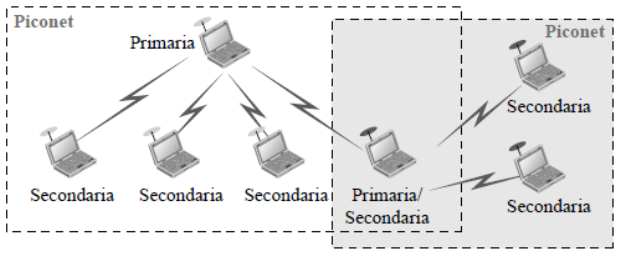
\includegraphics[width=9cm]{images/scatternet.PNG}
    \caption{Scatternet}
    \label{fig:scatternet}
\end{figure}

Un dispositivo Bluetooth ha un trasmettitore radio integrato a breve portata. La velocità di trasferimento dati corrente è 1 Mbps con ampiezza di banda da 2,4 GHz. Ciò significa che c'è una possibilità d'interferenza tra le LAN IEEE 802.11b wireless e le LAN Bluetooth.

Bluetooth usa una forma di TDMA come metodo d'accesso al mezzo. La stazione primaria e quelle secondarie comunicano tra loro usando degli slot temporali. La lunghezza di uno slot è 625 $\mu s$. Ciò significa che durante il tempo in cui una frequenza viene usata, una stazione primaria invia un frame a una secondaria, o viceversa. Da notare che la comunicazione è solo tra la primaria e una secondaria; le secondarie non possono comunicare direttamente l'una con l'altra.

Il Bluetooth usa una variante di TDMA, detta TDD-TDMA (TDMA duplex a divisione del tempo). II TDD-TDMA è un tipo di comunicazione half-duplex in cui il mettente e il destinatario inviano e ricevono dati, ma non contemporaneamente (half-duplex), tuttavia la comunicazione per ogni direzione usa diversi hop.

\begin{itemize}
    \item \textit{Comunicazione singola-secondaria.} Se la piconet ha una sola stazione secondaria, il funzionamento del TDMA è molto semplice. Il tempo viene diviso in slot da 625 $\mu s$. La stazione primaria usa gli slot a numeri pari (0, 2, 4, ...); la secondaria a numeri dispari (1, 3, 5, ...). Il TDD-TDMA consente alla primaria e alla secondaria di comunicare in modalità half-duplex. Nello slot 0 la primaria invia e la secondaria riceve; nello slot 1 la secondaria invia e la primaria riceve. Il ciclo viene ripetuto.

    \begin{figure}[ht]
        \centering
        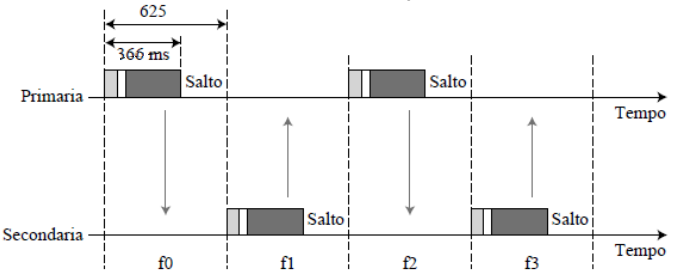
\includegraphics[width=9cm]{images/secondaria-singola.PNG}
        \caption{Comunicazione singola-secondaria}
        \label{fig:secondaria-singola}
    \end{figure}

    \item \textit{Comunicazione multipla-secondaria.} Il processo è un po' più complesso se ci sono più stazioni secondarie nella piconet. Anche in questo caso la primaria usa gli slot a numeri pari, mentre una secondaria trasmette nello slot a numero dispari successivo se il pacchetto della primaria nello slot precedente era indirizzato ad essa. Tutte le secondarie ascoltano gli slot a numeri pari, ma solo una secondaria trasmette in uno slot a numeri dispari.

    \begin{figure}[ht]
        \centering
        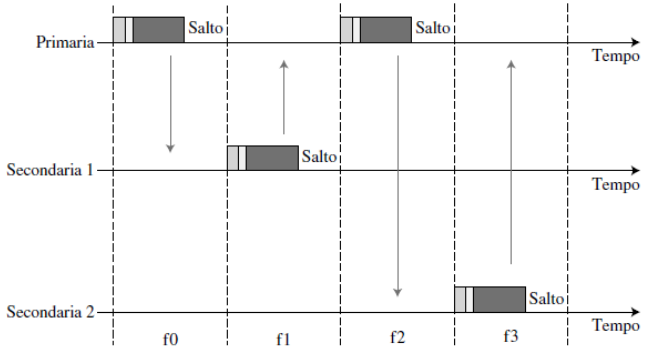
\includegraphics[width=9cm]{images/secondaria-multipla.PNG}
        \caption{Comunicazione multipla-secondaria}
        \label{fig:secondaria-multipla}
    \end{figure}

    \begin{enumerate}
        \item Nello slot 0 la primaria invia un frame alla secondaria 1.
        \item Nello slot 1 solo la secondaria 1 invia un frame alla primaria in quanto il frame precedente era indirizzato alla secondaria 1, le altre secondarie restano mute.
        \item Nello slot 2 la primaria invia un frame alla secondaria 2.
        \item Nello slot 3 solo la secondaria 2 invia un frame alla primaria in quanto il frame precedente era indirizzato alla secondaria 2, le altre secondarie sono mute.
        \item Il ciclo continua.
    \end{enumerate}
    
    Possiamo dire che questo metodo d'accesso è simile a un'operazione interrogazione/selezione con prenotazioni. Quando la primaria seleziona una secondaria, la interroga. Lo slot successivo è prenotato affinché la stazione interrogata possa inviare il suo frame. Se la secondaria interrogata non ha frame da inviare il canale resta inutilizzato.
\end{itemize}

\section{Accesso al mezzo mediante suddivisione del canale}
Nelle reti wireless, come le reti cellulari e quelle satellitari, vengono utilizzati dei meccanismi di accesso al mezzo trasmissivo basati sulla suddivisione del canale.

La channelization (o suddivisione del canale) è un metodo ad accesso multiplo nel quale l'ampiezza di banda disponibile di un link viene suddivisa in tempo, frequenza o codice, tra diverse stazioni. In questa sezione parleremo di tre protocolli di suddivisione del canale: FDMA, TDMA e CDMA.

\subsection{Frequency-Division Multiple Access (FDMA)}
Nel Frequency-Division Multiple Access (FDMA), o accesso multiplo a divisione di frequenza, l'ampiezza di banda disponibile viene divisa in bande di frequenza. Ad ogni stazione viene assegnata una banda per trasmettere i suoi dati. In altre parole ogni banda è riservata a una stazione specifica e appartiene sempre a tale stazione. Ogni stazione usa anche un filtro passa banda per limitare le frequenze del trasmettitore. Per evitare le interferenze della stazione, le bande assegnate vengono separate una dall'altra tramite piccole bande di guardia.

\begin{figure}[ht]
    \centering
    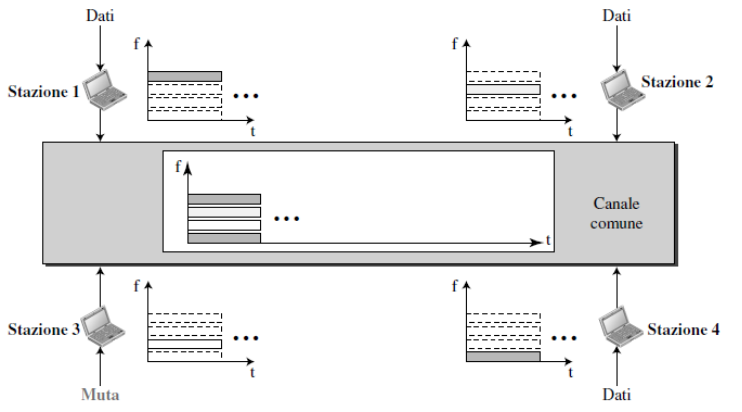
\includegraphics[width=11cm]{images/fdma.PNG}
    \caption{Accesso multiplo a divisione di frequenza (FDMA)}
    \label{fig:fdma}
\end{figure}

L'FDMA specifica una banda di frequenza predeterminata per l'intero periodo della comunicazione. Ciò significa che stream di dati (un flusso continuo di dati che non possono essere racchiusi in pacchetti) possono usare l'FDMA. 

Dobbiamo sottolineare che l'FDMA è un protocollo del livello di collegamento, e non deve essere confuso con un processo di multiplex, quello a divisione di frequenza (FDM), che in realtà è l'implementazione dell'FDMA al livello fisico.

\subsection{Time Division Multiple Access (TDMA)}
Nel Time-Division Multiple Access (TDMA), o accesso multiplo a divisione del tempo, le stazioni condividono l'ampiezza di banda del canale nel tempo. A ogni stazione viene assegnato uno slot di tempo durante il quale può inviare i dati. Ogni stazione trasmette i suoi dati nello slot che le è stato assegnato.

\begin{figure}[ht]
    \centering
    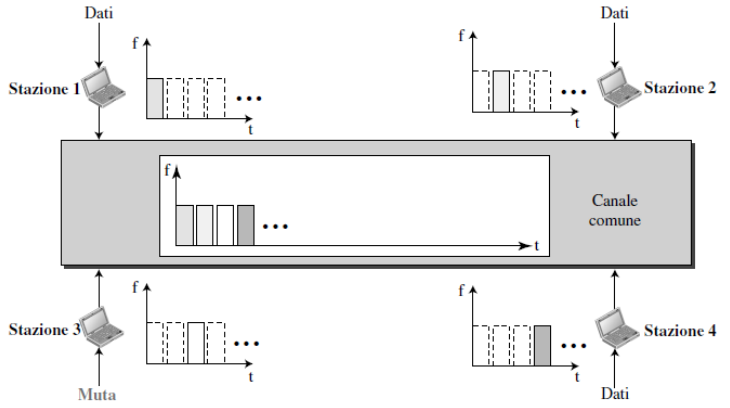
\includegraphics[width=11cm]{images/tdma.PNG}
    \caption{Accesso multiplo a divisione di tempo (TDMA)}
    \label{fig:tdma}
\end{figure}

Il problema principale con il TDMA sta nella sincronizzazione tra le varie stazioni. Ogni stazione deve conoscere l'inizio e la posizione del suo slot. Ciò può essere difficile a causa dei ritardi di propagazione introdotti nel sistema se le stazioni sono sparse in un'area ampia. Per compensare tali ritardi possiamo inserire dei tempi di guardia. La sincronizzazione normalmente viene realizzata tramite dei bit di sincronizzazione (normalmente chiamati bit preambolo) all'inizio di ogni slot.

Dobbiamo sottolineare che anche se il TDMA e il TDM (multiplex a divisione del tempo) sembrano concettualmente la stessa cosa, ci sono delle differenze tra di loro. Il TDM è una tecnica di livello fisico che unisce i dati dai canali più lenti e li trasmette usando un canale più veloce. Il processo usa un multiplexer fisico che inserisce delle unità dati da ogni canale. Il TDMA, d'altro canto, è un metodo d'accesso nel livello di collegamento. Questo livello in ogni stazione dice al suo livello fisico di usare lo slot che gli è stato assegnato. Non c'è multiplexer fisico al livello di collegamento.

\subsection{Code-Divison Multiple Access (CDMA)}
Il CDMA differisce dall'FDMA in quanto un solo canale occupa l'intera ampiezza di banda del link. Differisce dal TDMA in quanto tutte le stazioni possono inviare dati contemporaneamente, non essendoci suddivisione del tempo.

Per capire il CDMA facciamo un'analogia. CDMA significa semplicemente comunicazione con codici diversi. Per esempio in una stanza grande con molta gente, due persone possono parlare in inglese se nessun altro lo capisce. Altre due persone possono parlare cinese se sono gli unici due che comprendono tale lingua e così via. In altre parole il canale comune, lo spazio della stanza in questo caso, può facilmente consentire la comunicazione tra varie coppie, ma in lingue diverse (codici).

\begin{Example}{Idea della comunicazione con codice}{}
    Supponiamo di avere quattro stazioni, 1, 2, 3 e 4, collegate allo stesso canale. I dati dalla stazione 1 sono $d_1$, quelli dalla stazione 2 sono $d_2$, e cosi via. Il codice assegnato alla prima stazione è $c_1$, quello assegnato alla seconda è $c_2$, e cosi di seguito. Supponiamo che i codici assegnati abbiano due proprietà.
    \begin{enumerate}
        \item Se moltiplichiamo ogni codice per un altro otteniamo 0.
        \item Se moltiplichiamo ogni codice per sé stesso otteniamo 4 (il numero delle stazioni).
    \end{enumerate}

    Tenendo a mente queste due proprietà vediamo come le quattro stazioni sopra indicate possono inviare dei dati usando lo stesso canale comune.

    \begin{minipage}{\textwidth}
        \centering
        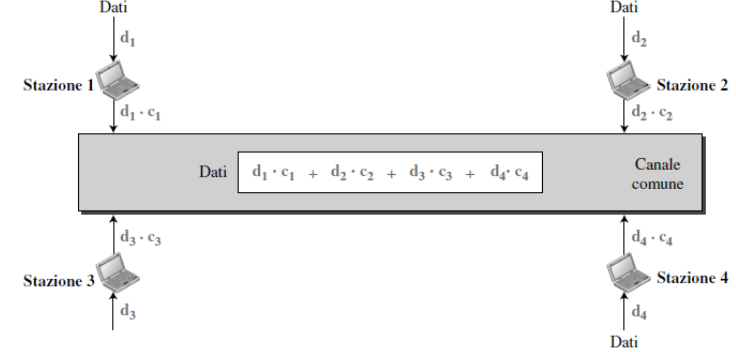
\includegraphics[width=0.8\textwidth]{images/cdma.PNG}
        %\captionof{figure}{Esempio}
    \end{minipage}

    La stazione 1 moltiplica (un tipo speciale di moltiplicazione, come vedremo) i suoi dati per il suo codice per ottenere $d_1\cdot c_1$. La stazione 2 moltiplica i suoi dati per il suo codice per ottenere $d_2\cdot c_2$, e così via. I dati che vanno sul canale sono la somma di tutti questi termini, come mostrato nel riquadro. Qualsiasi stazione che voglia ricevere dei dati da una delle altre tre stazioni moltiplica i dati sul canale per il codice del mittente. Per esempio, supponiamo che le stazioni 1 e 2 stiano parlando tra loro. La stazione 2 vuole sentire ciò che sta dicendo la 1. Essa moltiplica i dati sul canale per $c_1$, il codice della stazione 1. 
    
    Siccome ($c_1\cdot c_1$) fa 4, ma ($c_2\cdot c_1$), ($c_3\cdot c_1$) e ($c_4\cdot c_1$) sono tutti 0, la stazione 2 divide il risultato per 4 per ottenere i dati dalla stazione 1.
    \begin{align*}
        Dati=[(d_1\cdot c_1 + d_2\cdot c_2 + d_3\cdot c_3 + d_4\cdot c_4) \cdot c_1]/4\\
        =[d_1\cdot c_1\cdot c_1+d_2\cdot c_2\cdot c_1 + d_3\cdot c_3\cdot c_1 + d_4\cdot c_4\cdot c_1]/4=(4\times d_1)/4=d_1
    \end{align*}
\end{Example}

Il CDMA si basa sulla teoria della codifica. Ad ogni stazione viene assegnato un codice, che è una sequenza di numeri chiamati chip. La figura mostra i chip per l'esempio precedente. 

\begin{figure}[ht]
    \centering
    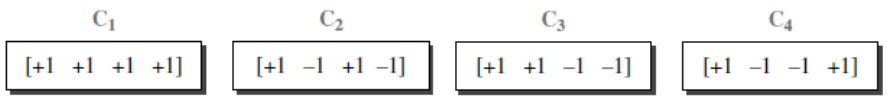
\includegraphics[width=11cm]{images/chip.PNG}
    \caption{Sequenze di chip}
    \label{fig:chip}
\end{figure}

Per ora dobbiamo sapere che le sequenze non vengono scelte in modo casuale, ma con molta attenzione. Vengono definite sequenze ortogonali e hanno le seguenti proprietà:
\begin{enumerate}
    \item Ogni sequenza è composta da $N$ elementi, dove $N$ è il numero di stazioni e deve essere una potenza di 2.
    \item Se moltiplichiamo una sequenza per un numero ogni elemento nella sequenza viene moltiplicato per tale numero. Ciò viene definito moltiplicazione di una sequenza per una scalare. Per esempio
    \begin{equation*}
        2\cdot[+1+1-1-1]=[+2+2-2-2]
    \end{equation*}
    Se moltiplichiamo due sequenze uguali, elemento per elemento, e sommiamo i risultati, otteniamo $N$, dove $N$ è il numero di elementi di ogni sequenza. Tale dato viene definito il prodotto interno di due sequenze uguali. Per esempio
    \begin{equation*}
        [+1+1-1-1]\cdot[+1+1-1-1]=1+1+1+1=4        
    \end{equation*}
    \item Se moltiplichiamo due sequenze diverse, elemento per elemento, e aggiungiamo i risultati, otteniamo 0. Ciò viene chiamato prodotto interno di due diverse sequenze. Per esempio
    \begin{equation*}
        [+1+1-1-1]\cdot[+1+1+1+1]=1+1-1-1=0        
    \end{equation*}
    \item Sommare due sequenze significa aggiungere gli elementi corrispondenti. Il risultato è un'altra sequenza. Per esempio
    \begin{equation*}
        [+1+1-1-1]+[+1+1+1+1]=[+2+2+0+0]        
    \end{equation*}
\end{enumerate}

La codifica avviene in base ad alcune regole: se una stazione deve inviare il bit 0, essa lo codifica come -1, se deve inviare il bit 1, lo codifica come +1. Quando una stazione è inattiva, non invia alcun segnale, il che viene interpretato come uno 0.

\begin{figure}[ht]
    \centering
    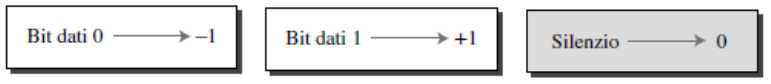
\includegraphics[width=11cm]{images/dati-cdma.PNG}
    \caption{Rappresenzazione dei dati nel CDMA}
    \label{fig:dati-cdma}
\end{figure}

\begin{Example}{Condivisione del canale nel CDMA}{}
    Come semplice esempio mostriamo come quattro stazioni condividono il link durante un intervallo da 1 bit. La procedura si può ripetere facilmente per altri intervalli. Supponiamo che le stazioni 1 e 2 stiano inviando un bit 0 e la stazione 4 stia trasmettendo un bit 1. La stazione 3 è muta. I dati sul sito mittente vengono tradotti in 1,-1,0 e +1. Ogni stazione moltiplica il numero corrispondente per il suo chip (la sua sequenza ortogonale), che è unica per ogni stazione. Il risultato è una nuova sequenza che viene inviata al canale. Per semplicità supponiamo che tutte le stazioni inviino le sequenze risultanti contemporaneamente. La sequenza sul canale è la somma di tutte e quattro le sequenze sopra definite.

    Ora immaginiamo che la stazione 3, che abbiamo detto essere muta, stia ascoltando la stazione 2. La stazione 3 moltiplica i dati totali sul canale per il codice per la stazione 2, che c[1 - 1 + 1 - 1] per ottenere
    \begin{gather*}
        [-1-1-3+1]\cdot[+1-1+1-1]=-4\\-4/4=-1\to \textit{bit } 0    
    \end{gather*}
    
    Il processo può essere meglio compreso se mostriamo il segnale digitale prodotto da ogni stazione e i dati recuperati a destinazione. La figura mostra i segnali corrispondenti per ogni stazione e il segnale che si trova sul canale comune.

    \begin{minipage}{\textwidth}
        \centering
        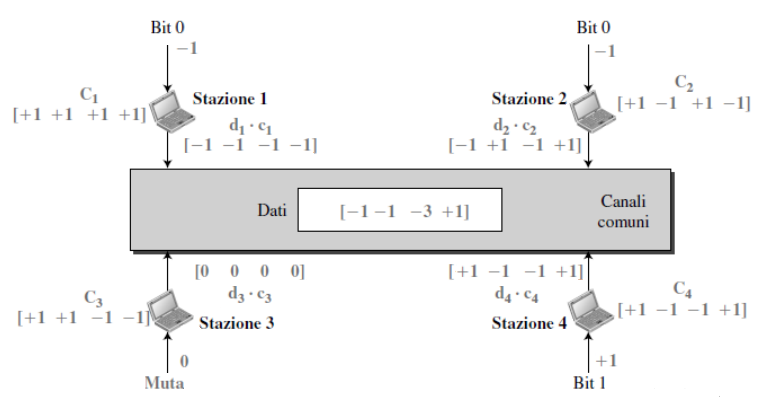
\includegraphics[width=0.8\textwidth]{images/condivisone-canale-cdma.PNG}
        %\captionof{figure}{Esempio}
    \end{minipage}

    La figura mostra come la stazione 3 possa rilevare i dati inviati dalla stazione 2 usando il codice per tale stazione. I dati totali sul canale vengono moltiplicati (operazione prodotto interno) per il segnale che rappresenta il codice chip della stazione 2 per ottenere uno nuovo segnale. La stazione quindi integra e somma l'area sotto il segnale, per ottenere il valore -4, che viene diviso per 4 ed interpretato come bit 0.

    \begin{minipage}{\textwidth}
        \centering
        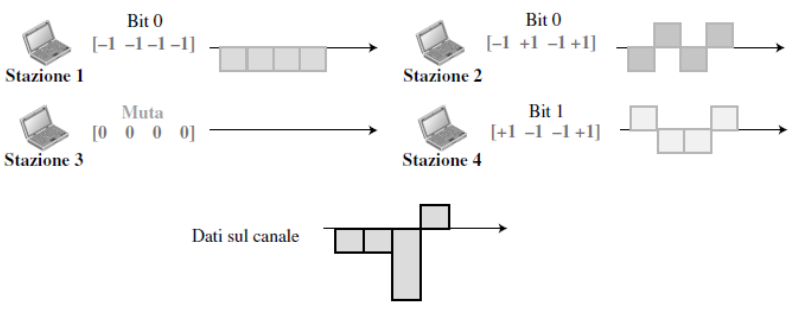
\includegraphics[width=0.8\textwidth]{images/segnale-stazioni.PNG}
        %\captionof{figure}{Esempio}
    \end{minipage}

    \begin{minipage}{\textwidth}
        \centering
        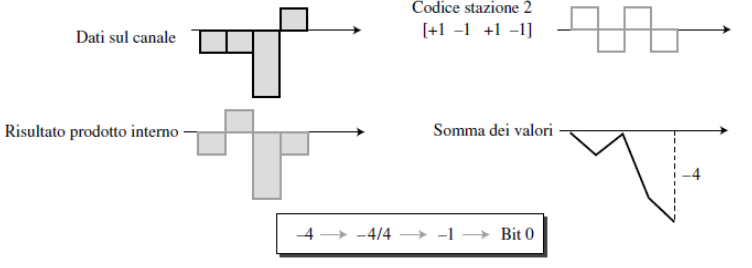
\includegraphics[width=0.8\textwidth]{images/decodifica-segnale.PNG}
        %\captionof{figure}{Esempio}
    \end{minipage}
\end{Example}

Per generare delle sequenze di chip usiamo una tabella di Walsh, una tabella bidimensionale con un numero uguale di righe e colonne.

\begin{figure}[ht]
    \centering
    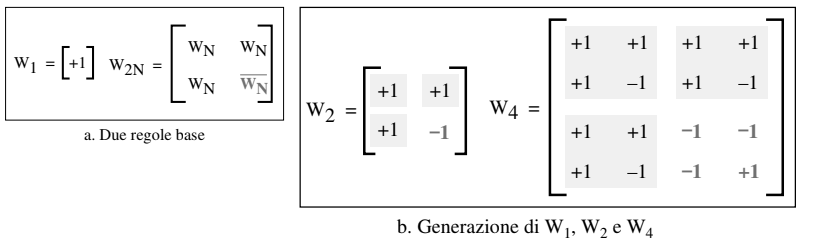
\includegraphics[width=11cm]{images/tabella-walsh.PNG}
    \caption{Regola generale ed esempi di creazione di tabelle di Walsh}
    \label{fig:tabella-walsh}
\end{figure}

Nella tabella di Walsh, ogni riga è una sequenza di chip. $W_1$ indica una sequenza da un chip con una riga e una colonna. Possiamo scegliere -1 o +1 per il chip di questa tabella a titolo esemplificativo (scegliamo +1). Secondo tale tabella se conosciamo quella per $N$ sequenze $W_{N}$ possiamo crearne un'altra per $2N$ sequenze $W_{2N}$. Il $W_{N}$ indicato con una barra superiore indica il complemento di $W_{N}$ in cui ogni +1 viene cambiato in -1 e viceversa. Viene mostra anche come possiamo creare $W_2$ e $W_4$ da $W_{1}$. Dopo aver selezionato $W_1$, $W_2$ può essere composto da quattro $W_{1}$ con l'ultimo che fa da complemento a $W_{1}$. Dopo che è stato generato $W_{2}$, si può creare $W_{4}$ da quattro $W_2$, con l'ultimo che fa da complemento a $W_{2}$. Naturalmente $W_{8}$ è composto da quattro $W_{4}$ e cosi via. Da notare che dopo aver creato $W_{N}$ ad ogni stazione viene assegnato un chip che cornsponde a una riga.

Il numero di sequenze $N$ deve essere una potenza di 2. In altre parole dobbiamo avere $N=2^m$.